\chapter{Biologi Struktur Protein}\label{ch:b3:structural-biology}

Max Perutz memulai kerjanya pada struktur hemoglobin tahun 1937 lalu
menerbitkannya tahun 1960: dua puluh dua tahun untuk melihat, pada \omterm{def:b3:structural-biology:methods}{daya pisah}
setengah nanometer, bagaimana empat rantai berisi seratus lima puluh asam
amino melipat mengelilingi empat hem. Sebuah molekul hemoglobin melipat
dirinya sendiri dalam beberapa milidetik. Di antara kedua kenyataan itu
terletak pokok bab ini: apa itu bentuk sebuah protein, mengapa rantai asam
amino memiliki satu bentuk dan bukan bentuk yang lain, bagaimana rantai itu
menemukan bentuknya begitu cepat di antara sekian banyak pilihan yang
jumlahnya astronomis, apa yang salah ketika ia tak menemukannya, bagaimana
bentuknya dilihat --- dengan sinar-X, dengan resonansi magnetik, dengan
elektron, dan kini dengan komputasi --- dan bagaimana sebuah protein bergerak di antara
bentuk untuk menjalankan kerjanya, dengan sakelar hemoglobin antara bentuk
tegang dan bentuk kendur sebagai model bagi setiap protein alosterik sesudahnya.

\section{Apa itu struktur sebuah protein}

\begin{definition}[Tingkat struktur]\label{def:b3:structural-biology:levels}
\index{struktur sekunder}\index{heliks alfa}\index{lembar beta}%
\index{struktur tersier}\index{domain}\index{lipatan}
\emph{Struktur primer} adalah urutan residunya. \emph{Struktur sekunder}
adalah konformasi setempat tulang punggungnya yang teratur, yang dimantapkan
ikatan hidrogen antara karbonil dan amida tulang punggungnya: \emph{heliks
$\alpha$}, sebuah spiral kanan berisi $3.6$ residu tiap putaran, yang naik
\qty{0.15}{nm} tiap residu (\qty{0.54}{nm} tiap putaran), dengan tiap
karbonilnya berikatan dengan amida empat residu di depannya; dan
\emph{lembar $\beta$}, yang untai terjulurnya berbaring bersisian, sejajar
atau berlawanan arah, berikatan dengan tetangganya, dengan rantai sampingnya
berselang-seling di atas dan di bawah lembarnya. \emph{Struktur tersier}
adalah lipatan satu rantai utuh dalam tiga dimensi; satuan mampat sepanjang
\numrange{50}{250} residu di dalamnya yang melipat secara mandiri disebut
sebuah \emph{domain}, dan tatanan unsur sekunder sebuah domain disebut
\emph{lipatannya}. \emph{Struktur kuaterner} adalah rakitan beberapa rantai:
$\alpha_{2}\beta_{2}$ pada hemoglobin. Sekitar \num{1300} lipatan menjelaskan
seluruh domain yang dikenal, dan beberapa lusin di antaranya --- lipatan
Rossmann, tong TIM, dan lipatan imunoglobulin --- menjelaskan sebagian
besar protein: alam memakai ulang lipatan lalu meragamkan urutannya.
\end{definition}

\begin{omfigure}
\begin{tikzpicture}
\begin{axis}[
  width=6.4cm, height=6.4cm,
  xmin=-180, xmax=180, ymin=-180, ymax=180,
  xlabel={$\phi$ (derajat)}, ylabel={$\psi$ (derajat)},
  xlabel style={font=\small}, ylabel style={font=\small},
  tick label style={font=\scriptsize}, xtick={-180,-90,0,90,180}, ytick={-180,-90,0,90,180},
  axis lines=box, grid=major, grid style={gray!25},
  clip=false,
]
% beta region
\fill[omDef!30] (axis cs:-180,90) rectangle (axis cs:-45,180);
\fill[omDef!30] (axis cs:-180,-180) rectangle (axis cs:-45,-150);
\node[font=\scriptsize, omDef!60!black] at (axis cs:-112,165) {untai $\beta$};
% alpha R region
\fill[omThm!30] (axis cs:-160,-70) rectangle (axis cs:-45,0);
\node[font=\scriptsize, omThm!70!black] at (axis cs:-105,-58) {$\alpha$ berputar kanan};
% alpha L region
\fill[omMeth!30] (axis cs:45,0) rectangle (axis cs:100,80);
\node[font=\scriptsize, omMeth!60!black, align=center] at (axis cs:72,40) {berputar\\kiri};
\addplot[only marks, mark=*, mark size=1pt, black] coordinates {(-57,-47)};
\node[font=\scriptsize, anchor=south west] at (axis cs:-52,-44) {$\alpha$: $(-57,-47)$};
\addplot[only marks, mark=*, mark size=1pt, black] coordinates {(-139,135)};
\node[font=\scriptsize, anchor=west] at (axis cs:-134,135) {$\beta$ berlawanan arah};
\end{axis}
\node[align=left, font=\scriptsize, anchor=west] at (7.0,3.0) {Kedua sudut puntir tulang punggung tiap\\residu, $\phi$ (terhadap N--C$_\alpha$) dan $\psi$ (terhadap\\C$_\alpha$--C), dibatasi benturan sterik\\pada daerah berwarna. Sebuah heliks menaruh tiap\\residu pada satu titik; sebuah untai, dekat titik lain.\\Glisina, tanpa rantai samping, menjangkau lebih jauh;\\prolina, dengan cincinnya, terpaku dekat $\phi = -60$.};
\end{tikzpicture}

{\small Diagram Ramachandran. Daerah yang diarsir adalah gabungan sudut
tulang punggung $\phi$ dan $\psi$ yang diizinkan secara sterik; heliks $\alpha$
berputar kanan dan untai $\beta$ masing-masing bersesuaian dengan satu daerah
kecil, dan sebagian besar residu protein yang terlipat jatuh pada salah
satunya.}
\end{omfigure}

\begin{proposition}[Apa yang menahan sebuah lipatan]\label{prop:b3:structural-biology:forces}
\index{efek hidrofob}\index{kemantapan tipis}
Protein yang terlipat dimantapkan oleh \emph{\omterm{prop:b3:structural-biology:forces}{efek hidrofob}} --- yaitu
menguburkan rantai samping nonpolar di dalam sebuah inti yang jauh dari air,
yang membebaskan molekul air yang kalau tidak akan tertata di sekelilingnya ---
oleh ikatan hidrogen \omterm{def:b3:structural-biology:levels}{struktur sekundernya} dan ikatan hidrogen gugus polar yang
terkubur, oleh pengemasan van der Waals sebuah inti sepadat kristal, oleh
jembatan garam sesekali, dan, pada protein yang disekresikan, oleh ikatan
disulfida. \omterm{prop:b3:structural-biology:forces}{Efek hidrofob} memasok sebagian besar dorongannya; ikatan
hidrogennya sebagian besar membayar dirinya sendiri (tulang punggung yang
berikatan dengan air pada keadaan tak terlipat berikatan dengan dirinya sendiri
pada keadaan terlipat) dan sebagai gantinya menentukan \omterm{def:b3:structural-biology:levels}{lipatan} yang \emph{mana}.
Energi bebas neto pelipatannya kecil, $\Delta G \approx -20$ sampai
\qty{-60}{kJ/mol} --- sekuat segenggam ikatan hidrogen bagi molekul yang
memiliki ratusan --- karena hilangnya entropi konformasi pada pelipatan
hampir meniadakan perolehan entalpinya. Protein bersifat \emph{mantap tipis}:
beberapa derajat, perubahan pH, atau satu mutasi pada intinya dapat
membuka \omterm{def:b3:structural-biology:levels}{lipatannya}, dan ketipisan itulah yang membuatnya dapat bergerak.
\end{proposition}

\begin{proof}[Bukti eksperimental]
Anfinsen (1961) membuka \omterm{def:b3:structural-biology:levels}{lipatan} ribonuklease~A dengan urea dan zat pereduksi,
sehingga memutus keempat disulfidanya dan memusnahkan keaktifannya; begitu
keduanya dibuang, enzimnya melipat kembali, lalu membentuk ulang keempat
pasangan disulfida yang benar dari $105$ pasangan yang mungkin, lalu memulihkan
keaktifannya sepenuhnya. Tak ada cetakan, tak ada enzim, tak ada keterangan di
luar urutannya yang hadir: struktur asalnya adalah keadaan yang paling mantap
secara termodinamika yang terjangkau rantainya, dan urutannya menyandikannya.
Mengoksidasi ulang disulfidanya selagi rantainya masih di dalam urea memberi
campuran teracak dengan keaktifan \qty{1}{\%}, yang lalu terurai menjadi
bentuk asalnya ketika dibiarkan melipat: rantainya menemukan minimumnya sendiri.
\end{proof}

\section{Bagaimana sebuah rantai menemukan lipatannya}

\begin{theorem}[Paradoks Levinthal]\label{thm:b3:structural-biology:levinthal}
\index{paradoks Levinthal}\index{corong pelipatan}
Andaikan tiap dari $n$ residu sebuah protein dapat mengambil $k$ konformasi
tulang punggung secara bebas, rantainya akan memiliki $k^{n}$ konformasi.
Dengan $k = 3$ dan $n = 100$ jumlahnya $3^{100} \approx
5\times 10^{47}$; mencuplik semuanya pada satu tiap pikodetik ($10^{12}$ tiap
detik) akan memakan $5\times 10^{35}$ detik, kira-kira $10^{28}$ tahun.
Protein seukuran itu melipat dalam hitungan milidetik sampai detik. Karena itu
pelipatannya bukan penelusuran acak atas konformasinya: permukaan energinya
sebuah \emph{corong}, yang di dalamnya hampir setiap konformasi sebagian
condong ke arah keadaan asalnya, dan rantainya menuruninya lewat langkah
setempat yang rata-rata menurun.
\end{theorem}
\begin{proof}
Cacahnya adalah asas perkalian; waktunya adalah cacahnya dibagi laju
cupliknya, $5\times 10^{47}/10^{12} = 5\times
10^{35}$ s, dan setahun sebesar $3\times 10^{7}$ s. Kesimpulannya adalah
kontrapositifnya: penelusuran acak sebesar itu mustahil dalam waktu yang
teramati, sehingga penelusurannya tidak acak. Yang membuatnya tidak acak
adalah bahwa interaksi yang terbentuk pada satu bagian rantainya bertahan
selagi bagian lain terbentuk (keruntuhan hidrofob dan pembentukan heliks
terjadi dalam hitungan mikrodetik lalu menciutkan ruang yang harus
ditelusuri), dan bahwa struktur yang sebagian benar rata-rata berenergi lebih
rendah daripada yang salah, sehingga penurunannya terpandu --- sebuah corong,
bukan lapangan golf dengan satu lubang.
\end{proof}

\begin{omfigure}
\begin{tikzpicture}[every node/.style={font=\scriptsize}, >=stealth]
  % funnel outline
  \draw[very thick, omDef] (-4,3) .. controls (-3.2,1.5) and (-1.2,0.2) .. (-0.35,-1.2) -- (-0.35,-1.6);
  \draw[very thick, omDef] (4,3) .. controls (3.2,1.5) and (1.2,0.2) .. (0.35,-1.2) -- (0.35,-1.6);
  \draw[very thick, omDef] (-0.35,-1.6) -- (0.35,-1.6);
  % rugged inner lines
  \draw[omDef!60, thick] (-3.3,2.6) .. controls (-2.9,2.2) and (-2.6,2.6) .. (-2.2,2.0) .. controls (-1.9,1.5) and (-1.7,1.9) .. (-1.4,1.2) .. controls (-1.1,0.7) and (-0.9,0.9) .. (-0.6,0.2);
  \draw[omDef!60, thick] (3.3,2.6) .. controls (2.9,2.1) and (2.5,2.5) .. (2.1,1.8) .. controls (1.8,1.3) and (1.5,1.6) .. (1.2,1.0) .. controls (1.0,0.6) and (0.8,0.8) .. (0.6,0.2);
  % axes
  \draw[->] (-5.9,-1.8) -- (-5.9,3.2) node[above, align=center] {energi\\bebas};
  \draw[<->] (-3.9,3.85) -- (3.9,3.85) node[midway, above] {entropi konformasi (lebar ansambelnya)};
  % labels
  \node[above] at (0,3.05) {rantai tak terlipat: banyak konformasi, energi tinggi};
  \node[right, align=left] at (3.3,1.4) {perangkap setempat: zat antara\\yang sebagian salah lipat};
  \node[left, align=right] at (-3.3,1.4) {keruntuhan cepat dan\\struktur sekunder};
  \node[below] at (0,-1.7) {keadaan asal: satu konformasi, energi terendah};
  \draw[->, thick, omThm] (-2.8,2.4) .. controls (-2.0,1.2) and (-0.8,0.5) .. (-0.15,-1.3);
  \node[omThm, left] at (-1.5,-0.5) {sebuah lintasan pelipatan};
\end{tikzpicture}

{\small \omterm{thm:b3:structural-biology:levinthal}{Corong pelipatan}. Energi bebasnya turun dan cacah konformasi yang
tersedia menciut seiring rantainya mendekati keadaan asalnya; dindingnya
berkerut, sehingga sebuah rantai dapat terperangkap di dalam zat antara yang
sebagian salah lipat, tetapi kemiringan keseluruhannya membawanya turun dalam
hitungan milidetik.}
\end{omfigure}

\begin{definition}[Pendamping]\label{def:b3:structural-biology:chaperones}
\index{pendamping}\index{Hsp70}\index{kaperonin}\index{GroEL}
Sebuah \emph{pendamping molekul} adalah protein yang membantu pelipatan
protein lain tanpa menjadi bagiannya dan tanpa memasok keterangan tentang
\omterm{def:b3:structural-biology:levels}{lipatannya}: pendamping itu mencegah penggumpalan yang bersaing dengan
pelipatan di dalam sitoplasma yang sesak. \emph{Hsp70} mengikat segmen
hidrofob yang terpapar pada rantai nasen atau rantai tak terlipat, lalu
melepaskannya pada hidrolisis ATP demi percobaan berikutnya; \emph{kaperonin}
GroEL (Hsp60 di dalam mitokondria, TRiC di dalam sitosol eukariot) adalah tong
ganda berisi empat belas subunit yang rongga pusatnya, yang ditudungi GroES,
mengurung satu rantai sampai \qty{60}{kDa} secara tersendiri selama kira-kira
sepuluh detik --- sebuah sangkar Anfinsen --- lalu melontarkannya entah
terlipat entah tidak, agar mencoba lagi. Sekitar sepersepuluh protein bakteri
yang baru dibuat melewati GroEL, dan sel yang pendampingnya kewalahan --- oleh
panas, dan itulah sebabnya sebagian besar disebut \emph{protein kejut panas}
yang diimbas naiknya suhu --- terisi gumpalan.
\end{definition}

\begin{definition}[Amiloid]\label{def:b3:structural-biology:amyloid}
\index{amiloid}\index{silang-beta}\index{prion}\index{penyakit salah lipat}
\emph{Amiloid} adalah gumpalan protein yang teratur, yang rantainya bertumpuk
menjadi fibril tak bercabang selebar \qtyrange{5}{10}{nm}, dengan untai tiap
rantainya berjalan tegak lurus terhadap sumbu fibrilnya dan berikatan hidrogen
dengan untai fibril berikutnya --- yaitu struktur \emph{silang-$\beta$}, yang
sama apa pun proteinnya. Hampir setiap protein dapat membentuknya pada keadaan
yang mengacaukan kemantapan; pada \emph{penyakit salah lipat} protein tertentu
melakukannya di dalam tubuh: amiloid-$\beta$ dan tau pada penyakit Alzheimer,
$\alpha$-sinuklein pada penyakit Parkinson, huntingtin, transtiretin, dan
amiloid pulau pada diabetes tipe~2. Sebuah \emph{prion} adalah amiloid yang
merambat: bentuk salah lipat protein prion PrP mengubah bentuk normalnya
begitu bersentuhan menjadi lebih banyak dirinya sendiri, sehingga
``infeksinya'' tidak mengusung asam nukleat, hanya sebuah bentuk --- yakni
mekanisme skrapi, ensefalopati spongiform sapi, dan penyakit
Creutzfeldt--Jakob, yang ditegakkan Prusiner sejak 1982 melawan perlawanan panjang.
\end{definition}

\begin{omfigure}
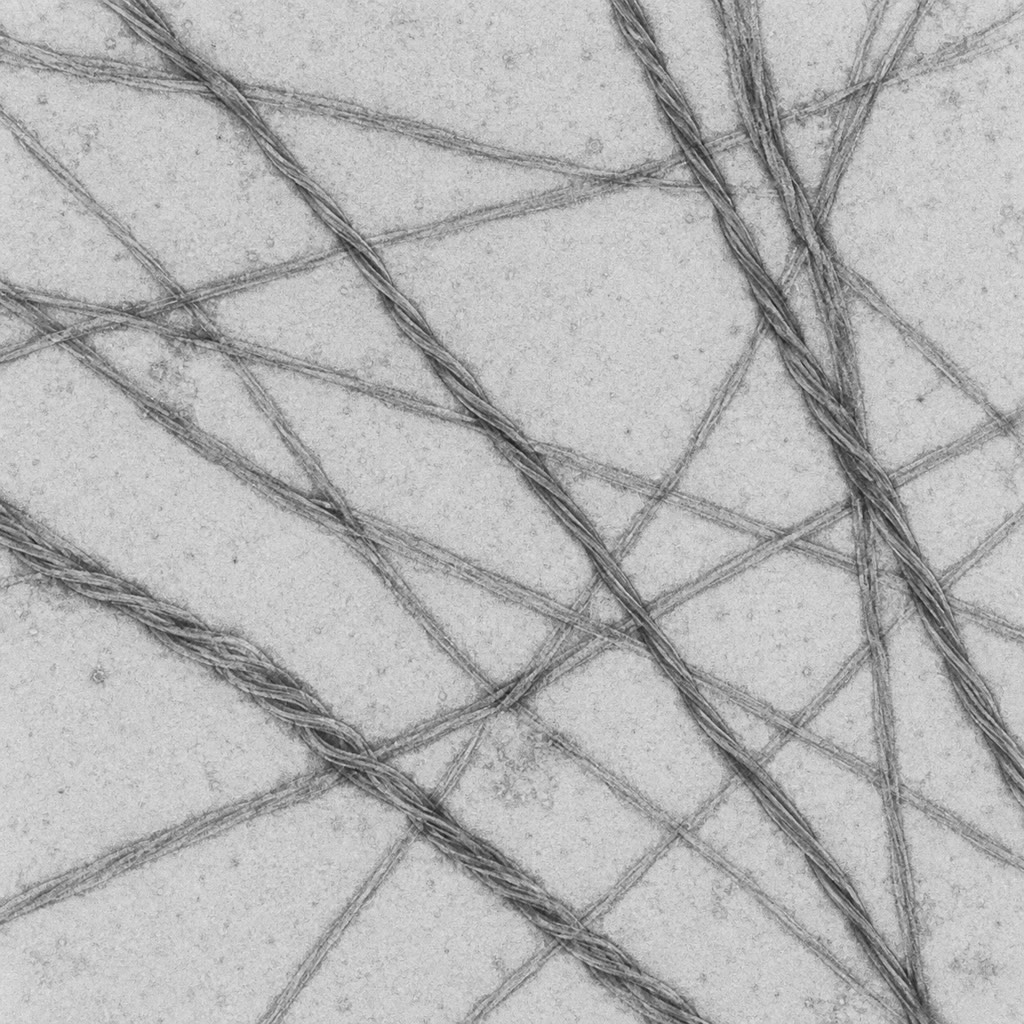
\includegraphics[width=0.36\linewidth]{images/book5/ai/b5-07-amyloid-fibrils.jpg}\hspace{0.04\linewidth}
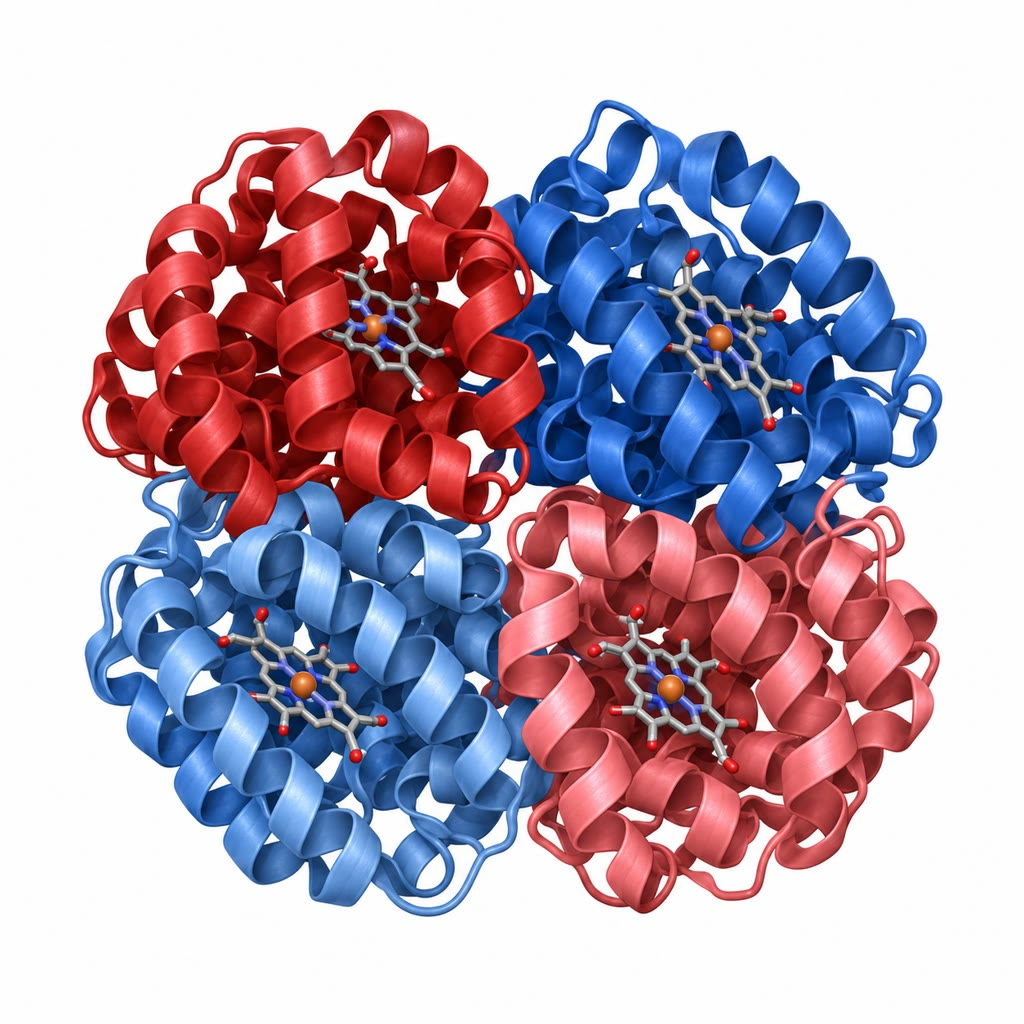
\includegraphics[width=0.36\linewidth]{images/book5/ai/b5-07-haemoglobin-model.jpg}

{\small Kiri: fibril \omterm{def:b3:structural-biology:amyloid}{amiloid} di bawah mikroskop elektron --- lurus, tak
bercabang, kadang-kadang terpilin, dan serupa strukturnya apa pun protein
penyusunnya. Kanan: tetramer hemoglobin, dua rantai $\alpha$ dan dua rantai
$\beta$, yang masing-masing memangku sebuah hem.}
\end{omfigure}

\section{Melihat sebuah protein}

\begin{definition}[Metode struktur]\label{def:b3:structural-biology:methods}
\index{kristalografi sinar-X}\index{spektroskopi NMR}%
\index{mikroskopi elektron krio}\index{daya pisah}
\emph{Kristalografi sinar-X} menumbuhkan sebuah kristal proteinnya,
memaparkannya pada berkas sinar-X, lalu merekam pola difraksinya; kedudukan
bintiknya memberi kisinya dan keamatannya, begitu fase gelombangnya
dipulihkan, memberi kerapatan elektron sel satuannya, dan ke dalamnya
rantainya dibangun. \emph{Resonansi magnetik inti} (NMR) mengukur, di dalam
larutan, kopling antarinti atom yang berdekatan di ruang, dan dari situ jarak
serta sebuah struktur dihitung; cara itu berhasil bagi protein di bawah
kira-kira \qty{40}{kDa} dan melaporkan geraknya. \emph{Mikroskopi elektron
krio} mencitra ribuan sampai jutaan molekul tunggal yang dibekukan di dalam
lapisan tipis es kaca, masing-masing pada orientasi acak, lalu menyusun ulang
kerapatan tiga dimensinya dengan menggabungkannya; sejak detektor elektron
langsung (2013) cara itu mencapai daya pisah atom dan tak menuntut kristal,
sehingga kompleks besar, protein membran, dan rakitan lentur yang tak pernah
mengkristal kini dipecahkan secara rutin. \emph{Daya pisah} sebuah struktur
adalah jarak terkecil ketika dua ciri masih terpisahkan: pada \qty{0.35}{nm}
tulang punggung dan rantai samping yang besar ditempatkan, pada
\qty{0.2}{nm} setiap atom, pada \qty{0.1}{nm} hidrogennya.
\end{definition}

\begin{proof}[Bukti eksperimental]
Kendrew (1958) memperoleh struktur protein yang pertama, yaitu mioglobin paus
sperma, pada \qty{0.6}{nm} --- sebuah sosis yang tak disangka-sangka tak
teratur, ``lebih rumit dan kurang setangkup daripada ramalan siapa pun''
--- dan pada \qty{0.2}{nm} tahun 1960, ketika heliks $\alpha$ yang diusulkan
Pauling dari pemodelan tahun 1951 terlihat untuk pertama kalinya.
Perutz (1960) memecahkan hemoglobin pada \qty{0.55}{nm} dengan
metode atom berat yang dirancangnya untuk memperoleh fasenya: atom raksa yang
dilekatkan pada proteinnya mengubah keamatannya dengan cara yang menyingkapkan
keterangan yang hilang. Dengan membandingkan bentuk beroksigen dan tak
beroksigen (1970) ia melihat subunitnya berputar satu sama lain sebesar
\qty{15}{\degree} saat mengikat oksigen, yakni peralihan alosterik pertama
yang teramati pada skala atom.
\end{proof}

\begin{omfigure}
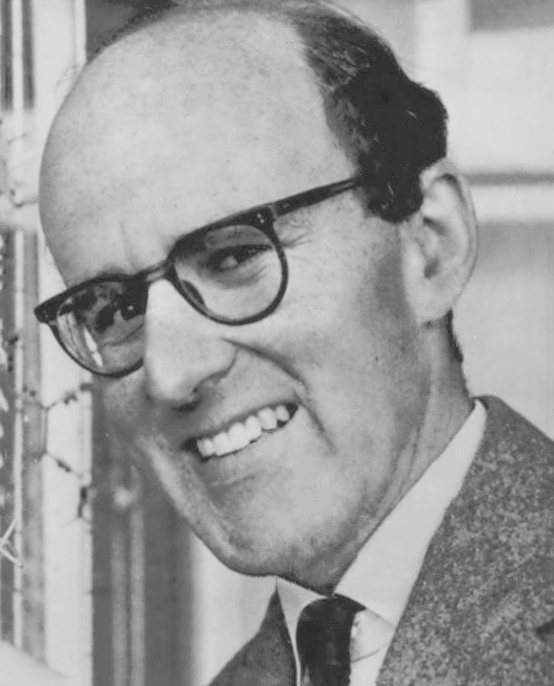
\includegraphics[width=0.30\linewidth]{images/book5/perutz.jpg}\hspace{0.04\linewidth}
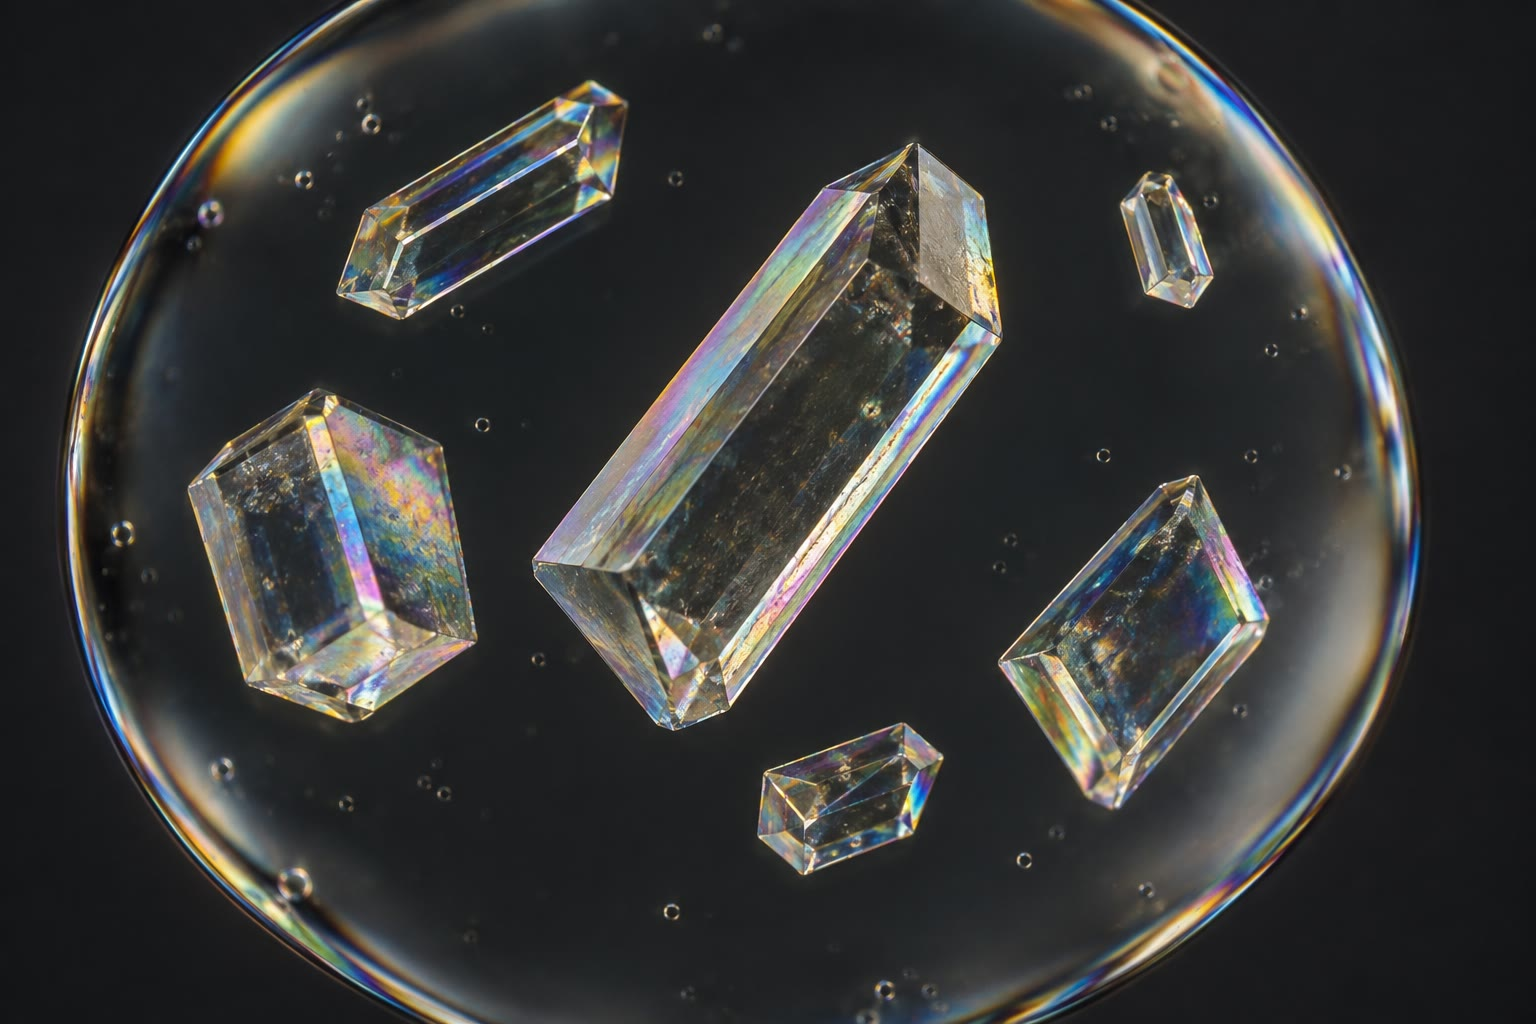
\includegraphics[width=0.30\linewidth]{images/book5/ai/b5-07-protein-crystals.jpg}\hspace{0.04\linewidth}
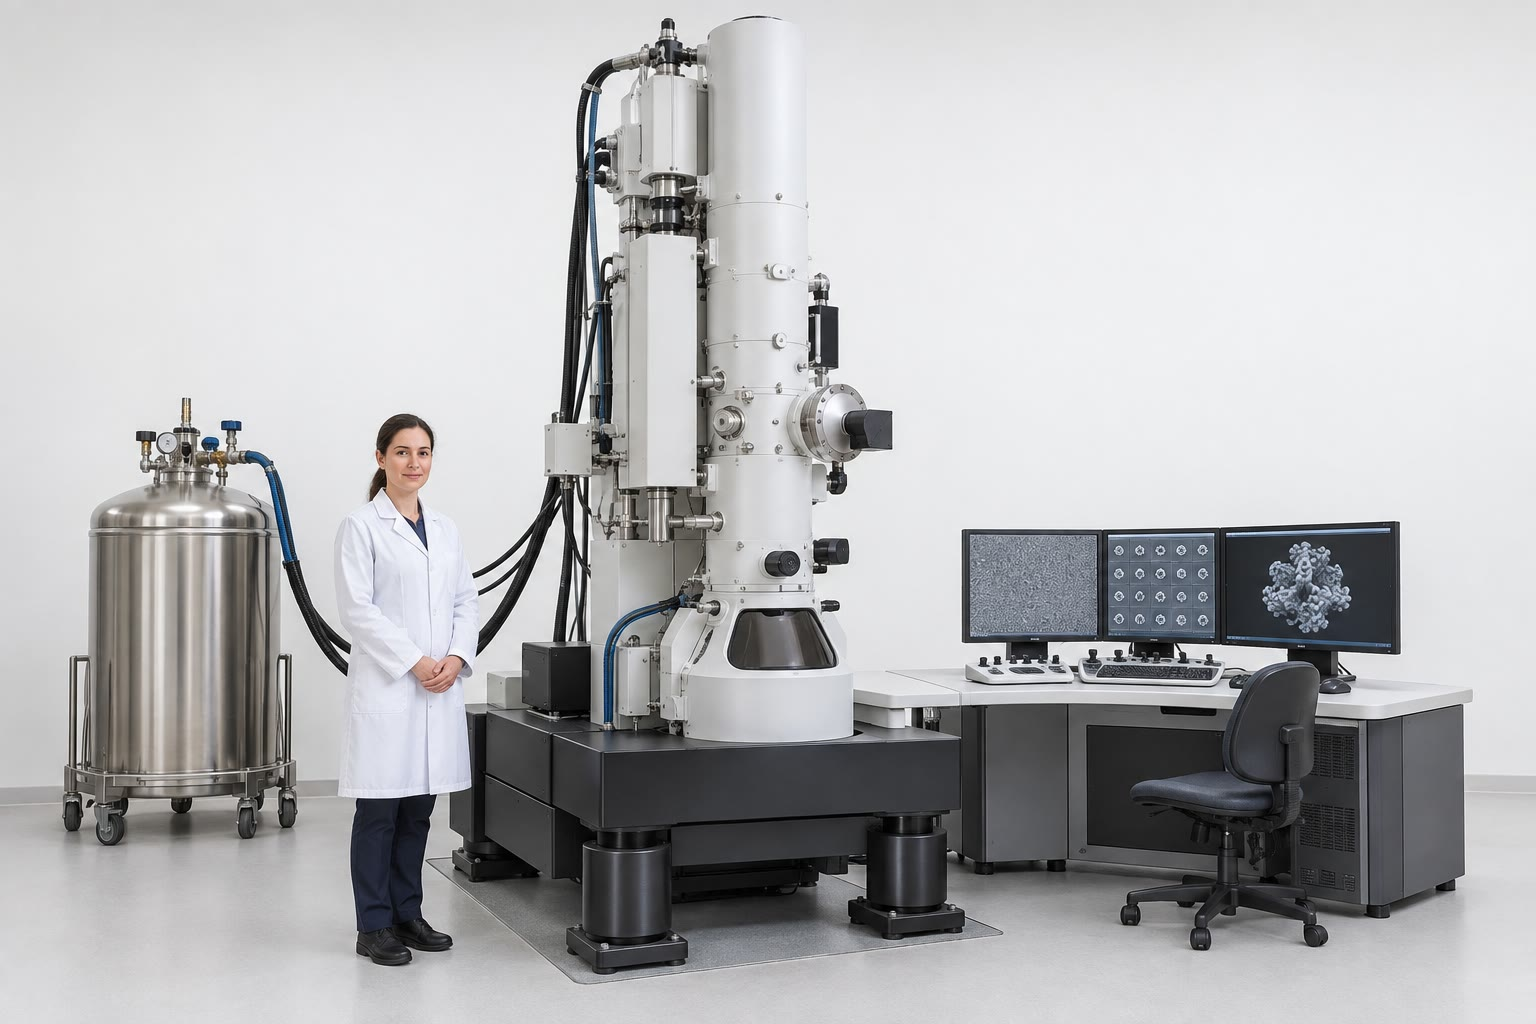
\includegraphics[width=0.30\linewidth]{images/book5/ai/b5-07-cryo-em.jpg}

{\small Max Perutz pada tahun 1962, tahun hadiah Nobelnya bagi
struktur hemoglobin (Associated Press, domain publik). Tengah:
kristal protein di dalam tetesan gantung, yaitu titik awal
kristalografi. Kanan: sebuah mikroskop elektron krio, yaitu instrumen
yang membuat kristal tak lagi diperlukan.}
\end{omfigure}

\begin{method}[Memecahkan sebuah struktur lewat kristalografi]\label{met:b3:structural-biology:crystallography}
\index{hukum Bragg}\index{masalah fase}
(1) Murnikanlah proteinnya sebanyak beberapa miligram lalu tapislah ratusan
keadaan (zat pengendap, pH, garam) untuk memperoleh kristal; (2) bekukanlah
sebuah kristal secara kilat lalu kumpulkanlah citra difraksinya di sebuah
sinkrotron selagi kristal itu berputar di dalam berkasnya; (3) indekskanlah
bintiknya untuk memperoleh sel satuan dan kesetangkupannya; sudut terbesar
ketika bintiknya masih terlihat menetapkan \omterm{def:b3:structural-biology:methods}{daya pisahnya} lewat \omterm{met:b3:structural-biology:crystallography}{hukum Bragg}, $d =
\lambda/(2\sin\theta)$; (4) pecahkanlah \emph{\omterm{met:b3:structural-biology:crystallography}{masalah fase}} --- detektornya
merekam keamatan tetapi bukan fase --- lewat atom berat, lewat hamburan anomali
selenium di dalam selenometionina, atau, bagi protein yang mirip protein yang
telah dikenal, lewat penggantian molekul, yakni menaruh model yang telah
dikenal di dalam selnya; (5) hitunglah kerapatan elektronnya, bangunlah
rantainya ke dalamnya, lalu haluskan modelnya terhadap datanya sampai
ketaksesuaiannya (faktor $R$) kecil; (6) sahkanlah: geometrinya, pencilan
Ramachandran, dan kecocokannya dengan data yang tak dipakai menghaluskan
modelnya.
\end{method}

\begin{omfigure}
\begin{tikzpicture}[every node/.style={font=\scriptsize}, >=stealth]
  % crystal
  \draw[thick, fill=omDef!20] (0,0) -- (1.4,0) -- (1.9,0.6) -- (0.5,0.6) -- cycle; \draw[thick, fill=omDef!30] (0,0) -- (0.5,0.6) -- (0.5,1.6) -- (0,1.0) -- cycle; \draw[thick, fill=omDef!25] (0.5,0.6) -- (1.9,0.6) -- (1.9,1.6) -- (0.5,1.6) -- cycle;
  \node[below] at (0.95,-0.1) {kristal: $10^{12}$ molekul sebaris};
  % beam
  \draw[->, very thick, omThm] (-2.2,0.9) -- (-0.1,0.9); \node[above] at (-1.2,0.95) {sinar-X, $\lambda \approx \qty{0.1}{nm}$};
  % diffracted beams
  \foreach \a in {-25,-12,5,18,30} \draw[->, omThm, thick] (1.9,0.9) -- ++(\a:3.2);
  % detector
  \draw[thick] (5.2,-1.2) rectangle (5.6,3.0); \node[right, align=left] at (5.7,2.6) {detektor: bintik pada\\sudut $\theta$, dengan\\keamatan $I$};
  \foreach \y in {-0.6,-0.1,0.6,1.2,1.9,2.4} \fill[black] (5.4,\y) circle (0.06);
  % arrow to density
  \draw[->, very thick] (7.4,0.9) -- (8.6,0.9) node[midway, above, align=center] {fasenya\\dipulihkan};
  \node[right, align=left] at (8.7,1.4) {kerapatan elektron};
  \draw[omDef, thick] (8.8,0.4) .. controls (9.1,1.1) and (9.5,0.2) .. (9.8,0.8) .. controls (10.1,1.3) and (10.4,0.3) .. (10.7,0.9);
  \node[right, align=left] at (8.7,-0.4) {model dibangun ke dalamnya,\\dihaluskan, disahkan};
  % Bragg
  \node[anchor=north west, align=left] at (-2.2,-0.7) {Bragg: $2d\sin\theta = \lambda$ ---\\$\theta$ terbesar yang teramati menetapkan daya pisah $d$};
\end{tikzpicture}

{\small Dari kristal ke model. Kisi yang teratur menghamburkan sinar-X menjadi
bintik yang terpisah; bintik pada sudut terbesar menetapkan \omterm{def:b3:structural-biology:methods}{daya pisahnya};
memulihkan fasenya mengubah keamatannya menjadi peta kerapatan elektron, dan
ke dalamnya rantainya dibangun.}
\end{omfigure}

\begin{remark}[Peramalan telah bergabung dengan metodenya]\label{rem:b3:structural-biology:prediction}
Sejak tahun 2020 struktur sebuah protein diramalkan dari urutannya dengan
kesaksamaan yang kerap menyaingi struktur percobaan \qty{0.3}{nm}
(\cref{ch:b3:bioinformatics}). Ramalannya adalah hipotesis tentang keadaan
asal yang statis; metode percobaannya tetap menjadi hakim, dan menjadi
satu-satunya sumber keterangan mengenai ligan, perubahan konformasi, dan
kompleks, serta dinamika yang dibahas di bawah ini. Perannya telah berubah --- sebuah model
ramalan memecahkan \omterm{met:b3:structural-biology:crystallography}{masalah fase} lewat penggantian molekul, dan mengarahkan
percobaan mana yang layak dikerjakan --- alih-alih yang satu menggantikan yang
lain.
\end{remark}

\section{Alosteri: hemoglobin sebagai modelnya}

\begin{definition}[Alosteri dan kekooperatifan]\label{def:b3:structural-biology:allostery}
\index{alosteri}\index{kekooperatifan}\index{koefisien Hill}%
\index{keadaan T}\index{keadaan R}
Sebuah protein disebut \emph{alosterik} apabila pengikatan sebuah ligan pada
satu tapak mengubah kegemaran tapak yang lain, lewat perubahan konformasi yang
diteruskan melintasi molekulnya. Ketika kedua tapaknya mengikat ligan yang
sama dan pengaruhnya positif, pengikatannya disebut \emph{kooperatif}:
kejenuhan pecahannya $Y$ naik terhadap kepekatan ligannya sebagai sigmoid,
bukan sebagai hiperbola, dan diperikan secara empiris oleh \emph{persamaan
Hill} $Y = [S]^{n_{H}}/(K^{n_{H}} +
[S]^{n_{H}})$ dengan \emph{koefisien Hill} $n_{H} > 1$ (hemoglobin:
$n_{H} \approx 2.8$ bagi keempat tapaknya; mioglobin, satu tapak: $n_{H} =
1$). Hemoglobin hadir dalam dua konformasi kuaterner, yaitu
\emph{keadaan T} (tegang, kegemarannya rendah, dipihak ketika tak ada oksigen
terikat) dan \emph{keadaan R} (kendur, kegemarannya tinggi), dan beralih di
antara keduanya sebagai satu kesatuan; proton, karbon dioksida, dan
2,3-bisfosfogliserat memantapkan T sehingga menurunkan kegemarannya --- yaitu
\omterm{prop:b3:structural-biology:mechanism}{efek Bohr}, yang membuat jaringan yang bekerja, asam dan hangat, mengambil
lebih banyak oksigen dari darahnya.
\end{definition}

\begin{theorem}[Model Monod--Wyman--Changeux]\label{thm:b3:structural-biology:mwc}
\index{model Monod--Wyman--Changeux}\index{model serentak}
Misalkan sebuah protein berisi $n$ tapak yang identik hadir dalam dua
konformasi, $T$ dan $R$, dalam kesetimbangan $L = [T_{0}]/[R_{0}]$ tanpa
ligan, dengan tiap tapak $R$ mengikat ligannya dengan tetapan disosiasi
$K_{R}$ dan tiap tapak $T$ dengan $K_{T}$, $c = K_{R}/K_{T} < 1$. Seluruh
tapak sebuah molekul beralih bersama-sama (peralihannya
\emph{serentak}). Maka dengan $\alpha = [S]/K_{R}$ kejenuhan pecahannya adalah
\[
Y = \frac{\alpha(1+\alpha)^{n-1} + Lc\alpha(1+c\alpha)^{n-1}}
{(1+\alpha)^{n} + L(1+c\alpha)^{n}},
\]
dan bagian molekul yang berada pada keadaan $R$ adalah $\bar R =
(1+\alpha)^{n}/\bigl[(1+\alpha)^{n} + L(1+c\alpha)^{n}\bigr]$. Bagi $L
\gg 1$ dan $c \ll 1$ kurvanya sigmoid: ligan yang pertama mengikat molekul $R$
yang langka dan bergemar tinggi lalu menjungkirkan kesetimbangannya, sehingga
pengikatannya merekrut lebih banyak $R$ dan kegemaran tapak yang tersisa pun
naik --- \omterm{def:b3:structural-biology:allostery}{kekooperatifan} tanpa interaksi langsung apa pun antartapak.
\end{theorem}
\begin{proof}
Spesi dengan $i$ ligan terikat pada bentuk $R$ berkepekatan
$[R_{0}]\binom{n}{i}\alpha^{i}$ (tiap dari $\binom{n}{i}$ pilihan tapak
terisinya menyumbang $([S]/K_{R})^{i}$ menurut hukum aksi massa), dan pada
bentuk $T$ berkepekatan $[T_{0}]\binom{n}{i}(c\alpha)^{i}$, karena
$[S]/K_{T} = c\alpha$. Dengan menjumlahkan atas $i$ lewat teorema binomial,
total proteinnya $[R_{0}]\bigl[(1+\alpha)^{n} + L(1+c\alpha)^{n}\bigr]$
dan total ligan yang terikat $[R_{0}]\sum_{i} i\binom{n}{i}\bigl[
\alpha^{i} + L(c\alpha)^{i}\bigr] = [R_{0}]\,n\bigl[\alpha(1+\alpha)^{n-1}
+ Lc\alpha(1+c\alpha)^{n-1}\bigr]$, dengan memakai $\sum_{i} i\binom{n}{i}x^{i} =
nx(1+x)^{n-1}$. Membagi ligan terikat dengan $n$ kali total proteinnya memberi
$Y$; bagian $R$-nya adalah suku $R$ dibagi totalnya. Ketika $\alpha$
kecil, suku $T$ mendominasi penyebutnya (karena $L \gg 1$) dan
$Y \approx c\alpha$, yakni kegemaran $T$ yang rendah; ketika $\alpha$ cukup besar
sehingga $(1+\alpha)^{n} > L(1+c\alpha)^{n}$, suku $R$ mengambil alih dan
kegemarannya menjadi $K_{R}$: peralihan antara kedua rezim itulah sigmoidnya.
\end{proof}

\begin{example}[Hemoglobin dalam angka]\label{ex:b3:structural-biology:hb-numbers}
Ambillah $n = 4$, $K_{R} = \qty{1}{mmHg}$, $c = 0.01$ (sehingga $K_{T} =
\qty{100}{mmHg}$) dan $L = 3\times 10^{5}$. Pada tekanan parsial
oksigen di dalam darah arteri, \qty{100}{mmHg}, $\alpha = 100$ dan $Y =
0.97$; pada \qty{40}{mmHg}, yakni nilai vena saat istirahat, $Y = 0.78$; pada
\qty{26}{mmHg}, $Y = 0.52$ --- modelnya menghasilkan ulang tekanan
setengah-jenuh \qty{26}{mmHg}; pada \qty{20}{mmHg}, di dalam otot yang
berolahraga, $Y = 0.35$. Sebuah pengusung tak kooperatif dengan tekanan
setengah-jenuh yang sama akan memberi $100/126 = 0.79$ di dalam paru-paru dan
$20/46 = 0.43$ di dalam ototnya, sehingga melepaskan $0.36$ kemampuannya di
tempat hemoglobin melepaskan $0.62$. \omterm{def:b3:structural-biology:allostery}{Kekooperatifan} itulah yang membuat sebuah
pengusung memuat penuh pada satu tekanan dan melepaskan sebagian besarnya
pada tekanan yang hanya lima kali lebih rendah.
\end{example}

\begin{omfigure}
\begin{tikzpicture}
\begin{axis}[
  width=0.7\linewidth, height=5.8cm,
  axis x line=bottom, axis y line=left,
  xmin=0, xmax=120, ymin=0, ymax=1.05,
  xlabel={tekanan parsial oksigen (mmHg)}, ylabel={kejenuhan $Y$},
  xlabel style={font=\small, at={(axis description cs:0.5,-0.12)}, anchor=north},
  ylabel style={font=\small},
  tick label style={font=\small}, xtick={0,20,40,60,80,100,120}, ytick={0,0.5,1},
  clip=false,
]
\addplot[very thick, omThm, domain=0.1:120, samples=120] {(x*(1+x)^3 + 300000*0.01*x*(1+0.01*x)^3)/((1+x)^4 + 300000*(1+0.01*x)^4)};
\addplot[very thick, omDef, domain=0:120, samples=60] {x/(x+26)};
\addplot[dashed, gray] coordinates {(26,0) (26,0.52)}; \addplot[dashed, gray] coordinates {(0,0.52) (26,0.52)};
\draw[gray, dashed] (axis cs:20,0) -- (axis cs:20,0.35); \draw[gray, dashed] (axis cs:100,0) -- (axis cs:100,0.97);
\node[font=\scriptsize, omThm, anchor=north west] at (axis cs:50,0.15) {hemoglobin (MWC, $n = 4$, $L = 3\times 10^{5}$, $c = 0.01$)};
\node[font=\scriptsize, omDef, anchor=north east] at (axis cs:118,0.72) {satu tapak, $P_{50}$ sama};
\node[font=\scriptsize, anchor=south] at (axis cs:20,1.0) {otot}; \node[font=\scriptsize, anchor=south] at (axis cs:100,1.0) {paru-paru};
\end{axis}
\end{tikzpicture}

{\small Kejenuhan oksigen hemoglobin yang dihitung dari persamaan
Monod--Wyman--Changeux dengan parameter contohnya
(merah), terhadap pengusung bertapak tunggal dengan tekanan setengah-jenuh
yang sama (biru). Antara paru-paru dan otot yang bekerja, pengusung yang
kooperatif melepaskan nyaris dua kali lebih banyak.}
\end{omfigure}

\begin{proposition}[Mekanisme sakelarnya]\label{prop:b3:structural-biology:mechanism}
\index{efek Bohr}\index{2,3-bisfosfogliserat}
Pada deoksihemoglobin, besinya duduk sedikit di luar bidang hemnya, tertarik
ke arah histidina proksimalnya, dan hemnya melengkung seperti kubah. Pengikatan
oksigen meratakan hemnya lalu menarik besinya, dan bersamanya histidina serta
heliks tempatnya berada, sejauh kira-kira \qty{0.06}{nm} ke arah
hemnya; pergeseran itu diperkuat pada antarmuka antara dimer
$\alpha_{1}\beta_{1}$ dan $\alpha_{2}\beta_{2}$, yang berputar sebesar
\qty{15}{\degree} lalu memutus jembatan garam yang menahan \omterm{def:b3:structural-biology:allostery}{keadaan T}.
Efektornya bekerja pada jembatan yang sama itu: proton mengikat histidina yang
jembatannya hanya ada pada T (yakni \omterm{prop:b3:structural-biology:mechanism}{efek Bohr}), karbon dioksida membentuk
karbamat dengan ujung aminonya sehingga memantapkan T, dan
2,3-bisfosfogliserat, molekul kecil yang sangat negatif, duduk di dalam rongga
pusat di antara rantai $\beta$-nya, yang hanya cukup lebar pada T. Hemoglobin
janin, yang rantai $\gamma$-nya kurang kuat mengikatnya, bergemar lebih tinggi
daripada milik ibunya sehingga menarik oksigen melintasi plasenta.
\end{proposition}

\section{Protein yang bergerak}

\begin{definition}[Ketakteraturan dan dinamika]\label{def:b3:structural-biology:disorder}
\index{protein tak teratur secara hakiki}\index{ansambel konformasi}%
\index{kondensat biomolekul}
Sebuah daerah yang \emph{tak teratur secara hakiki} tidak memiliki \omterm{def:b3:structural-biology:levels}{lipatan}
yang mantap sendirian dan hadir sebagai ansambel konformasi yang saling
berubah dengan cepat, dan kerap baru melipat ketika berjumpa mitranya; sekitar
sepertiga protein manusia mengusung daerah tak teratur sepanjang lebih dari
tiga puluh residu, dan daerah itu banyak terdapat pada pengisyaratan dan
pengaturan, tempat sebuah segmen lentur dapat difosforilasi pada banyak tapak,
mengikat beberapa mitra secara bergiliran, dan bertindak sebagai penghubung.
Protein yang terlipat pun bergerak: rantai sampingnya berputar dalam
pikodetik, lengkungnya membuka dalam nanodetik sampai mikrodetik, \omterm{def:b3:structural-biology:levels}{domainnya}
berengsel dalam mikrodetik sampai milidetik, dan daur katalitik sebuah enzim
adalah tarian gerak semacam itu, bukan gembok dan kunci yang statis. Sebuah
struktur kristal adalah satu jepretan sebuah \emph{ansambel konformasi}; NMR
dan simulasi molekul melihat sisanya. Protein dan RNA tak teratur yang
bervalensi banyak juga dapat memisah dari sitoplasma menjadi tetesan cair ---
\emph{kondensat biomolekul} seperti nukleolus, butiran cekaman, dan badan P ---
yang memekatkan reaksi tanpa membran, dan penuaannya menjadi gumpalan padat
merupakan salah satu jalan menuju penyakit \omterm{def:b3:structural-biology:amyloid}{amiloid}.
\end{definition}

\begin{remark}[Struktur dan fungsi]\label{rem:b3:structural-biology:sf}
Pelajaran enam puluh tahun struktur bersisi dua. Sebuah \omterm{def:b3:structural-biology:levels}{lipatan} adalah
pemecahan masalah fisik --- ikatlah ini, katalisilah itu, teruskanlah sebuah
isyarat sepanjang empat nanometer --- dan mengetahui strukturnya kerap membuat
mekanismenya terang, sebagaimana terjadi bagi besi hemnya dan bagi putaran
dimer hemoglobin yang didorong oksigen. Dan sebuah \omterm{def:b3:structural-biology:levels}{lipatan} adalah objek
sejarah: beberapa ratus arsitektur yang sama, yang diutak-atik, digandakan,
dan difusikan, melayani seluruh keragaman fungsi protein, sehingga struktur
sebuah protein bakteri kerap akan memberi tahu kita bagaimana sepupunya pada
manusia bekerja.
\end{remark}

\section{Latihan}

\begin{exercise}[$\star$]\label{exo:b3:structural-biology:1}
Definisikanlah keempat tingkat struktur protein lalu berikan contoh
masing-masing pada hemoglobin.
\end{exercise}

\begin{exercise}[$\star$]\label{exo:b3:structural-biology:2}
Sebuah heliks $\alpha$ memuat $36$ residu. Berapa panjangnya, berapa
putaran yang dibuatnya, dan berapa ikatan hidrogen tulang punggung yang
menahannya (karbonil tiap residu berikatan dengan amida empat residu di depannya)?
\end{exercise}

\begin{exercise}[$\star$]\label{exo:b3:structural-biology:3}
Apa yang ditunjukkan pelipatan ulang ribonuklease oleh Anfinsen, dan mengapa
penting mengerjakan percobaannya tanpa kehadiran komponen sel apa pun?
\end{exercise}

\begin{exercise}[$\star$]\label{exo:b3:structural-biology:4}
Urutkanlah kristalografi, NMR, dan \omterm{def:b3:structural-biology:methods}{mikroskopi elektron krio} menurut ukuran
protein yang paling baik ditangani masing-masing, lalu katakan mana yang
memberi keterangan tentang gerak.
\end{exercise}

\begin{exercise}[$\star\star$]\label{exo:b3:structural-biology:5}
Ulangilah cacahan Levinthal bagi protein berisi $150$ residu dengan $k = 2$,
dan bagi peptida berisi $20$ residu dengan $k = 3$. Bagi yang mana dari
keduanya penelusuran acak masih terbayangkan dalam satu detik pada $10^{12}$
percobaan tiap detik?
\end{exercise}

\begin{exercise}[$\star\star$]\label{exo:b3:structural-biology:6}
Dengan persamaan MWC dan $n = 2$, $L = 100$, $c = 0.01$, hitunglah
$Y$ pada $\alpha = 1$, $10$, dan $100$, lalu bandingkan dengan satu tapak
bertetapan disosiasi $K_{R}$ ($Y = \alpha/(1+\alpha)$). Di mana
\omterm{def:b3:structural-biology:allostery}{kekooperatifannya} tampak?
\end{exercise}

\begin{exercise}[$\star\star$]\label{exo:b3:structural-biology:7}
Jelaskanlah, dengan model MWC, mengapa 2,3-bisfosfogliserat menurunkan
kegemaran oksigen hemoglobin, parameter model yang mana yang diubahnya, dan
mengapa darah simpanan, yang kehilangan senyawa itu, buruk mengantarkan
oksigen ketika ditransfusikan.
\end{exercise}

\begin{exercise}[$\star\star$]\label{exo:b3:structural-biology:8}
Sebuah kristal berdifraksi sampai sudut maksimum $\theta = \qty{15}{\degree}$
dengan sinar-X berpanjang gelombang \qty{0.1}{nm}. Berapa \omterm{def:b3:structural-biology:methods}{daya pisahnya}? Ciri
protein yang mana yang akan terlihat? Sudut berapa yang dibutuhkan bagi
\qty{0.12}{nm}?
\end{exercise}

\begin{exercise}[$\star\star$]\label{exo:b3:structural-biology:9}
Sebuah mutasi mengganti leusina yang terkubur dengan lisina. Ramalkanlah
pengaruhnya pada kemantapannya, dengan \cref{prop:b3:structural-biology:forces},
lalu jelaskan mengapa penggantian yang sama pada permukaannya tak berbahaya.
Lalu jelaskanlah mengapa protein dengan $\Delta G_{\text{lipat}} =
\qty{-30}{kJ/mol}$ bukanlah protein yang ``sangat mantap'' walaupun angkanya
tampak besar.
\end{exercise}

\begin{exercise}[$\star\star\star$]\label{exo:b3:structural-biology:10}
Turunkanlah bagian molekul yang berada pada keadaan $R$, yaitu $\bar R$, dari
spesi yang dicacah pada bukti \cref{thm:b3:structural-biology:mwc},
lalu tunjukkan bahwa untuk $c \to 0$ kepekatan ligan ketika separuh
molekulnya berada pada $R$ memenuhi $(1+\alpha)^{n} = L$. Hitunglah
$\alpha$ ini bagi parameter hemoglobin lalu bandingkan dengan $P_{50}$.
\end{exercise}

\begin{exercise}[$\star\star\star$]\label{exo:b3:structural-biology:11}
\omterm{def:b3:structural-biology:amyloid}{Prion} meneruskan sebuah bentuk. Jelaskanlah mengapa hipotesis ``protein saja''
ditentang, percobaan apa yang akan membantahnya, dan bukti apa
(ketahanan daya infeksinya terhadap nuklease dan cahaya ultraungu,
kepekaannya terhadap zat pendenaturasi protein, \omterm{def:b3:structural-biology:amyloid}{prion} sintetik) yang
mendukungnya. Mengapa sebuah \omterm{def:b3:structural-biology:amyloid}{prion} menuntut benih?
\end{exercise}

\begin{exercise}[$\star\star\star$]\label{exo:b3:structural-biology:12}
Sebuah famili protein mempertahankan \omterm{def:b3:structural-biology:levels}{lipatannya} sementara urutannya menyimpang
sampai keidentikan \qty{15}{\%}. Jelaskanlah mengapa struktur lebih lestari
daripada urutan, residu macam apa yang menjadi residu yang lestari, dan
bagaimana hal itu dimanfaatkan baik oleh metode \omterm{def:b3:bioinformatics:msa}{profil}
(\cref{ch:b3:bioinformatics}) maupun oleh perancangan protein baru.
\end{exercise}

\section{Soal: Lipatan Sebuah Globin}

\begin{problem}[{Soal akhir pekan --- heliks sebuah globin yang diukur,
pelipatannya yang ditakar terhadap Levinthal, pengikatan oksigennya yang
dihitung dari model dua keadaan, dan strukturnya yang dipecahkan dari sebuah
kristal, berakhir pada selisih kejenuhan antara paru-paru dan otot, waktu
Levinthal, serta daya pisah petanya}]
\label{pb:b3:structural-biology:1}
Data: sebuah rantai globin berisi $150$ residu, massa residu rata-rata \qty{110}{Da},
\qty{75}{\%} residunya berada di dalam delapan heliks $\alpha$; kenaikan
heliksnya \qty{0.15}{nm} tiap residu, $3.6$ residu tiap putaran. Volume jenis
parsial proteinnya \qty{0.73}{cm^3/g}. Parameter MWC bagi hemoglobin:
$n = 4$, $K_{R} = \qty{1}{mmHg}$, $c = 0.01$, $L = 3\times 10^{5}$.
Panjang gelombang sinar-X \qty{0.1}{nm}; sel satuannya kubus berusuk \qty{6}{nm};
kristalnya kubus berusuk \qty{100}{\micro m}.

\medskip
\noindent\textbf{Bagian I --- Anatomi sebuah rantai.}
\begin{enumerate}
  \item Berapa residu yang berada di dalam heliks? Berapa panjang heliks
        seluruhnya, dan berapa putarannya?
  \item Berapa ikatan hidrogen tulang punggung yang dimuat heliksnya, bila
        dihitung satu tiap residu di luar empat residu pertama tiap heliks?
  \item Berapa massa rantainya dan berapa volumenya menurut volume jenis
        parsialnya; berapa jari-jari bola bervolume itu?
  \item Rantai yang terjulur akan sepanjang \qty{0.36}{nm} tiap residu.
        Bandingkanlah panjangnya dengan garis tengah bolanya: dengan faktor
        berapa pelipatannya memampatkan rantainya?
  \item Kedelapan heliksnya rata-rata $14$ residu. Andaikan residunya
        dijajarkan ujung ke ujung, berapa bagian panjang terjulurnya yang
        berupa heliks, dan bagaimana heliksnya memendekkannya?
  \item Sebuah globin mengubur sekitar $40$ rantai samping nonpolar di dalam
        intinya. Dengan mengambil \qty{4}{kJ/mol} pemantapan hidrofob tiap
        rantai samping yang terkubur dan ongkos entropi konformasi sebesar
        \qty{0.9}{kJ/mol} tiap residu pada pelipatan (seluruh $150$ residu),
        taksirlah $\Delta G$ neto pelipatannya lalu bandingkan dengan
        rentang pada \cref{prop:b3:structural-biology:forces}.
\end{enumerate}

\medskip
\noindent\textbf{Bagian II --- Menemukan \omterm{def:b3:structural-biology:levels}{lipatannya}.}
\begin{enumerate}[resume]
  \item Hitunglah cacahan Levinthal bagi $150$ residu dengan $k = 3$
        dan waktu untuk mencupliknya pada $10^{12}$ tiap detik.
  \item Globinnya melipat dalam \qty{10}{ms}. Berapa konformasi, paling
        banyak, yang dapat dikunjunginya? Berapa bagian cacahannya itu?
  \item Andaikanlah sebagai gantinya tiap heliks terbentuk secara bebas dalam
        \qty{1}{\micro s}, lalu kedelapan heliks yang terbentuk itu mencari
        pengemasannya di antara $8!$ urutan yang dicuplik pada $10^{6}$ tiap
        detik. Taksirlah waktu pelipatannya. Apakah ini sebuah corong?
  \item Sebuah \omterm{def:b3:structural-biology:chaperones}{kaperonin} mengurung sebuah rantai selama \qty{10}{s} tiap daur
        lalu melepaskannya dalam keadaan terlipat dengan peluang $0.3$ tiap
        daur. Berapa harapan cacah daurnya, dan berapa harapan waktunya,
        untuk melipat sebuah substrat yang sukar? Berapa bagiannya yang
        masih tak terlipat sesudah semenit?
  \item Sebuah mutasi yang mengacaukan kemantapan menaikkan bagian yang tak
        terlipat pada \qty{37}{\celsius} dari $10^{-4}$ menjadi $10^{-2}$.
        Dengan $\Delta G =
        -RT\ln(K)$ dan $K = [\text{terlipat}]/[\text{tak terlipat}]$, berapa
        besar perubahan $\Delta G_{\text{lipat}}$-nya?
  \item Jelaskanlah mengapa protein tak terlipat yang seratus kali lebih
        banyak dapat menjadi pembeda antara sehat dan penyakit \omterm{def:b3:structural-biology:amyloid}{amiloid},
        dengan memakai kebutuhan akan sebuah benih.
\end{enumerate}

\medskip
\noindent\textbf{Bagian III --- Mengikat oksigen.}
\begin{enumerate}[resume]
  \item Hitunglah $Y$ dari persamaan MWC pada $\alpha = 100$ (paru-paru) dan
        $\alpha = 20$ (otot yang bekerja).
  \item Hitunglah bagian molekul yang berada pada keadaan $R$ pada kedua
        tekanan itu.
  \item Berapa banyak oksigen yang dimuatnya yang dilepaskan antara paru-paru
        dan otot? Bandingkanlah dengan pengusung bertapak tunggal dengan
        tekanan setengah-jenuh \qty{26}{mmHg}.
  \item Darah mengusung \qty{150}{g} hemoglobin tiap liter, dan tiap gramnya
        mengikat \qty{1.34}{mL} oksigen. Berapa mililiter oksigen tiap liter
        yang diantarkan hemoglobin ke ototnya, menurut
        pertanyaan 15? Tubuh yang beristirahat memakai \qty{250}{mL/min}:
        berapa aliran darah yang dituntutnya saat istirahat (pelepasan dari
        $0.97$ menjadi $0.78$)?
  \item Bisfosfogliserat menaikkan $L$ menjadi $3\times 10^{6}$. Hitunglah
        ulang $Y$ pada $\alpha = 40$ lalu katakan apa akibatnya bagi
        pengantaran saat istirahat.
  \item Hemoglobin janin, pada dasarnya, memiliki $L = 3\times 10^{4}$.
        Hitunglah $Y$-nya pada tekanan plasenta \qty{30}{mmHg}, bandingkan
        dengan milik ibunya, lalu jelaskan pemindahannya.
\end{enumerate}

\medskip
\noindent\textbf{Bagian IV --- Melihatnya.}
\begin{enumerate}[resume]
  \item Berapa sel satuan yang dimuat kristalnya? Bila tiap selnya
        memuat empat rantai globin, berapa molekul yang berdifraksi bersama?
  \item Bintiknya terlihat sampai $\theta = \qty{14.5}{\degree}$. Berapa
        \omterm{def:b3:structural-biology:methods}{daya pisahnya}, dan apakah rantai sampingnya akan tertempatkan?
  \item Sudut berapa yang akan memberi \qty{0.15}{nm}? Mengapa kristal yang
        buruk keteraturannya hanya berdifraksi sampai sudut rendah?
  \item Pada \omterm{def:b3:structural-biology:methods}{mikroskopi elektron krio}, isyarat citra yang dirata-ratakan
        tumbuh sebagai akar kuadrat cacah partikelnya. Bila
        \num{10000} partikel memberi \qty{0.6}{nm}, dan \omterm{def:b3:structural-biology:methods}{daya pisahnya}
        membaik sebagai kebalikan isyaratnya, berapa partikel yang
        memberi \qty{0.3}{nm}?
  \item \omterm{def:b3:structural-biology:methods}{Mikroskopi elektron krio} tidak menuntut kristal. Sebutkanlah dua
        macam protein atau kompleks yang bagi keduanya hal itu menentukan
        apakah sebuah struktur dapat diperoleh sama sekali, lalu jelaskan
        sebabnya.
  \item Sebuah model ramalan globin itu berbeda dari struktur kristalnya
        sebesar \qty{0.1}{nm} rata-rata pada tulang punggungnya. Sebutkanlah
        dua hal yang tak dapat dipasok ramalannya sedangkan kristalnya dapat.
  \item Ringkaskanlah: pelepasan antara paru-paru dan otot (pertanyaan~15),
        waktu Levinthal bagi $150$ residu (pertanyaan~7), dan
        \omterm{def:b3:structural-biology:methods}{daya pisah} petanya (pertanyaan~20).
\end{enumerate}
\end{problem}
